\section{Problem Definition}
\label{sec:method}


\begin{figure*}[htb]
	\centering
	\includegraphics[width=0.45\linewidth]{images/formulation}
	\hspace{0.1\linewidth}
	\includegraphics[width=0.40\linewidth]{images/formulation2}
	\caption{Our generative model for joint registration and co-segmentation (a) and its associated graphical model (b). (a) illustrates 7 Gaussian models $\{\vb{x}_i, \Sigma_i\}^{7}_{i=1}$ are grouped into two object models $O_1$ and $O_2$. Each object is transformed to a point set $\vb{V}_i$ by $\phi_{mi}$. A 3{D} point in a point set $\vb{V}_m$ is a sampling point from a Gaussian mixture model composed of the 7 transformed Gaussian models. } 
	\label{fig:formulation}
\end{figure*}

In this section, we introduce our formulation of the joint registration and co-segmentation problem for point sets. 
%Tabel~\ref{tab:symbol} lists all the symbols used in our formulation. 
The input of our problem is a group of 3D point sets  $\mathcal{V}=\{\mathbf{V}_m\}^{M}_{m=1}$ that are captured at $M$ different times in a scene, where objects move in different ways. Each point set $\mathbf{V}_m=\{\mathbf{v}_{mi}\}^{L_m}_{i=1}$ contains $L_m$ 3D points. Our problem is to simultaneously partition the point sets into $N$ objects and figure out the transformations from objects to each point set. For partitioning, we output point-wise label vectors $\{\mathbf{y}_m\}$ for each input point set to indicate its object partition. For registration, we output $\{\mathbf{R}_{mn},\mathbf{t}_{mn}\}$ to indicate the transformations from $N$ objects to $M$ point sets, respectively.

\comments{
\begin{table}[!hbp]
\centering
\caption{Table of symbols used in the paper.} 
\label{tab:symbol}
\begin{tabular}{c|l}
\hline
Symbol         & Definition\\
\hline
$M$            & The number of input point sets.\\
$\mathbf{V}_m$ & The $m^{th}$ input point set.\\
$\mathcal{V}$  & The input point sets $\{\mathbf{V}_m\}^{M}_{m=1}$.\\
$L_m$          & The number of points of the $m^{th}$ point set $\mathbf{V}_m$.\\
$\mathbf{v}_{mi}$ & The $i^{th}$ point of $\mathbf{V}_m$.\\
$\mathbf f_{mi}$   & The point-wise feature vector of $\mathbf v_{mi}$.\\
$z_{mi}$       & The latent parameter for $\mathbf v_{mi}$.\\
               & $z_{mi}=k$ means $\mathbf{v}_{mi}$ is generated by $k^{th}$ Gaussian. \\
$\mathcal{Z}$            & $\mathcal{Z}=\{z_{mi}|m=1...M,i=1...L_m\}$.\\
$N$            & The number of objects in the scene.\\
$K_n$          & The number of Gaussian models for the $n^{th}$ object. \\
$K_S$		   & The sum of $\{K_1,K_2,\cdots,K_{n-1}\}$\\
			   & $K_S = \sum_{i=1}^{n-1}K_i$\\
$K_{all}$      & The total number of Gaussian models of all objects. \\
               & $K_{all} = \sum_{n=1}^N K_n $.\\
$p_k$          & The weight of $k^{th}$ Gaussian. $\sum_{k=1}^{K_{all}}p_k=1$.\\
$\mathbf x_k$     & The centroid of $k^{th}$ Gaussian model.\\
$\mathbf {x}^{v}_k$   & The centroid of $k^{th}$ Gaussian for point position.\\
$\mathbf {x}^{f}_k$   & The centroid of $k^{th}$ Gaussian for point feature.\\
$\Sigma_k$     & The covariance matrix of $k^{th}$ Gaussian model.\\
$\sigma_k$     & $\Sigma_k=\sigma_k^2\mathbf{I}$, where $\mathbf{I}$ is an identity matrix.\\
$\sigma^v_k$   & Gaussian covariance parameter for point position\\
$\sigma^f_k$   & Gaussian covariance parameter for point feature\\
$\phi_{mn}$    & Rigid transformation from object $O_n$ to point set $\mathbf{V}_m$.\\
%$\mathbf{R}_{mn}$ & The rotation matrix for $\phi_{mn}$.\\
%$\mathbf{t}_{mn}$ & The translation vector for $\phi_{mn}$.
\hline
\end{tabular}
\end{table}
}

\subsection{Basic Formulation}
For robustness, we do not model a point set as a simple composition of transformed 3D points in each object model. 
Instead, we model each point set as a realization of an unknown central Gaussian mixture model (GMM) from of the transformed object models. 
In other words, we explicitly separate total $K_{all}$ Gaussian models to $N$ groups to represent $N$ objects $\{O_n\}_{n=1}^N$ as
%
\begin{equation}
\begin{aligned}
\{
\underbrace{ \{\mathbf{x}_{1},\Sigma_{1}\}, \cdots, \{\mathbf{x}_{K_1},\Sigma_{K_1}\}  }_{O_1},&\underbrace{ \{\mathbf{x}_{K_1+1},\Sigma_{K_1+1}\}, \cdots, \{\mathbf{x}_{K_1+K_2},\Sigma_{K_1+K_2}\}  }_{O_2},\\ 
\cdots \cdots,& 
\underbrace{ \{\mathbf{x}_{K_S+1},\Sigma_{K_S+1}\},\cdots,\{\mathbf{x}_{K_S+K_n},\Sigma_{K_S+K_n}\}  }_{O_n},\cdots \}
\end{aligned}
\end{equation}
where $K_S = \sum_{i=1}^{n-1}K_i$.

The Gaussian centroids $\{\mathbf{x}_{k}\}$ represent the point positions in objects. $\{\Sigma_{k}\}$ quantify the variance of point positions in objects. $O_n$ has $K_n$ Gaussian models and $\{K_n\}_{n=1}^N$ are predefined, as described in Sec.~\ref{sec:imp}.
The total number of Gaussian centroids is denoted as $K_{all} = \sum_{n=1}^{N}K_n$.  
%
Each object $O_{n}$ is rigidly transformed to each point set $\mathbf{V}_m$ with a transformation $\phi_{mn}(\mathbf{x}_{k})=\mathbf{R}_{mn}\mathbf{x}_{k}+\mathbf{t}_{mn}$ for $\mathbf{x}_{k} \in O_n$.
%
Figure \ref{fig:formulation} shows a simple illustration for this formulation.
Hence, for each point $\mathbf{v}_{mi}$ in a point set $\mathbf{V}_m$, given object models $\{O_{n}\}$ and their rigid transformations $\{\phi_{mn}\}$ to the point sets, we can write
%
\begin{equation}
\label{equ:model}
P(\mathbf{v}_{mi})=\sum^{K_{all}}_{k=1}p_k\mathcal{N}(\mathbf{v}_{mi}|\phi_{mn}(\mathbf{x}_k),\Sigma_k),
\end{equation}
%
where the observed point $\mathbf{v}_{mi}$ is a sampling point from a large Gaussian mixture model that represents $N$ objects together.
%I move it here.
$\{p_k\}_{k=1}^{K_{all}} $ are weights for $K_{all}$ Gaussian models. 


Given the generative representation, the unknown parameters of our joint registration and segmentation problem are
%
\begin{equation}
\varTheta=\big \{\{p_k,\mathbf{x}_{k},\Sigma_k\}_{k=1}^{K_{all}},\{\phi_{mn}\}_{m=1,n=1}^{M,N}\big\}.
\end{equation}
%
Once we estimate these parameters, each point in all input point sets can be assigned to one of the Gaussian models according to the largest sampling probability.
%
Since the Gaussian models are predefined to be one of the $N$ objects, we can further deduce the $\{\mathbf{y}_m\}_{m=1}^M$ indicating vectors of object-level co-segmentation for each input point set based on such assignment.
%
To estimate the parameters $\Theta$ to fit all the input point sets without knowing object labels for all 3D points, the problem can be solved in an Expectation-Maximization (EM) framework. 
%
In particular, we bring in hidden variables as: 
\begin{equation}
\mathcal{Z}=\{z_{mi}|m=1...M,i=1...L_m\},
\end{equation}
%
such that $z_{mi}=k$, $k \in \{1,2...,K_{all}\}$ assigns the observed point $\mathbf{v}_{mi}$ to the $k^{th}$ Gaussian model $\vb{x}_k, \Sigma_k$. 
%
We aim to maximize the expected complete-data log-likelihood:
\begin{equation}
\label{equ:obj0}
\mathcal{E}(\Theta|\mathcal{V},\mathcal{Z})=\mathbb{E}_{\mathcal{Z}}[\ln P(\mathcal{V},\mathcal{Z};\Theta)|\defV]={\sum_{\mathcal{Z}}P(\defZ|\defV,\Theta)\ln{P(\mathcal{V},\mathcal{Z};\Theta)}}.
\end{equation}


This formulation can be seen as an adaption of the joint registration formulation in \cite{Evangelidis2014}, upon which we separate Gaussian models into groups to express multiple objects. 
%
%The parameter $\defZ$ that assigns observed points to Gaussian models can naturally indicate the object-level segmentation.
%
Under the assumption that the input points are independent and identically distributed, we can rewrite the objective defined in Eq.~(\ref{equ:obj0}) into:
%
\begin{equation} \label{equ:obj2}
\Theta=\arg\max\sum_{m,i,k}\alpha_{mik}\big(\ln p_k + \ln P(\mathbf{v}_{mi}|z_{mi}=k;\Theta)\big),
\end{equation}
%
where $\alpha_{mik} = P( z_{mi} = k | \mathbf{v}_{mi} ; \Theta )$.
%
By bringing in Eq.~(\ref{equ:model}) and ignoring constant terms, we can rewrite the objective as:
\begin{equation}
\label{equ:obj3}
\Theta=\arg\max\Big(-\frac{1}{2}\sum_{m,i,k}\alpha_{mik}\big(||\mathbf{v}_{mi}-\phi_{mn}(\mathbf{x}_k)||_{\Sigma_k}^2 + \ln |\Sigma_k| - 2\ln p_k\big)\Big), 
\end{equation}
%
where the $|\cdot|$ denotes the determinant and $||\mathbf{x}||_{\mathbf{A}}^2= \mathbf{x}^T\mathbf{A}^{-1}\mathbf{x}$. 
%
It is predefined that $\mathbf{x}_k$ is one of the Gaussian centroids used to represent the $n^{th}$ object, which is why we apply the transformation $\phi_{mn}$ on $\mathbf{x}_k$. 
%
For the convenience of computation, we restrict the model to isotropic covariances, i.e., $\Sigma_k=\sigma^2\mathbf{I}$ and $\mathbf{I}$ is an identity matrix.
%
Now, we can optimize the objective through iterating between estimating $\alpha_{mik}$ (Expectation-step) and maximizing $\mathcal{E}(\Theta|\defV,\defZ)$ with respect to each parameter in $\Theta$ (Maximization-step).

%These steps are:
\noindent\textbf{E-step}:
this step estimates the posterior probability $\alpha_{mik}$ of $\mathbf v_{mi}$ to be a point generated by the $k^{th}$ Gaussian model.
%
\begin{equation}
\label{equ:estep}
\alpha_{mik}=\frac{p_k\sigma_k^{-3}exp(-\frac{1}{2\sigma_k^2}||\mathbf v_{mi}-\phi_{mn}(\mathbf x_k)||^2)}{\sum_s^{K_{all}}p_s\sigma_s^{-3}exp(-\frac{1}{2\sigma_s^2}||\mathbf v_{mi}-\phi_{mn}(\mathbf x_s)||^2)}
\end{equation}
%

\noindent\textbf{M-step-a}: this step updates the transformations $\phi_{mn}$ that maximize $\mathcal{E}(\Theta)$, given instant values for $\alpha_{mik}$, $\mathbf{x}_k$, $\sigma_k$.
%
We only consider rigid transformations, making  $\phi_{mn}(\mathbf{x})=\mathbf{R}_{mn}\mathbf{x}+\mathbf{t}_{mn}$. The maximizer $\mathbf{R}_{mn}^*,\mathbf{t}_{mn}^*$ of $\mathcal{E}(\Theta)$ is the same with the minimizers of the following constrained optimization problems
%
\begin{equation}
\left\{
\begin{array}{rcl}
\min_{\mathbf{R}_{mn},\mathbf{t}_{mn}}&      &||(\mathbf{W}_{mn}-\mathbf{R}_{mn}\mathbf{X}_n-\mathbf t_{mn}\mathbf{e}^T)\Lambda_{mn}||_F^2\\
s.t.&      &\mathbf{R}_{mn}^T\mathbf{R}_{mn}=I, |\mathbf{R}_{mn}|=1\\
\end{array} \right.
\end{equation}
where $\Lambda_{mn}$ is a $K_n \times K_n$ diagonal matrix with elements $\lambda_{mnk}=\frac{1}{\sigma_k}\sqrt{\sum_i^{L_{m}}\alpha_{mik}}$, $L_m$ is the number of point for the $m^{th}$ input point set, $\mathbf{X}_n = [\mathbf{x}_{K_S+1}, \mathbf{x}_{K_S+2},...., \mathbf{x}_{K_S+K_n}]$ is the matrix stacked by the centroids of Gaussian models that are predefined to represent the $n^{th}$ object. 
$\mathbf{e}^T$ is a vector of ones, $||\cdot||_F$ denotes the Frobenius norm, and $\mathbf{W}_{mn}=[\mathbf{w}_{m(K_S+1)},\mathbf{w}_{m(K_S+2)},...,\mathbf{w}_{mk},...,\mathbf{w}_{m(K_S+K_n)}]$ where $\mathbf{w}_{mk}$ is a weighted average point as
%
\begin{equation}
\mathbf{w}_{mk}=\frac{\sum_{i=1}^{L_m}\alpha_{mik} \mathbf{v}_{mi}}{\sum_{i=1}^{L_m}\alpha_{mik}}
\end{equation}

This problem has a similar solution with \cite{Evangelidis2014}. 
The only difference is that we are estimating the transformation from Gaussian models to the input point sets instead of the transformation from input point sets to Gaussian models, since there are multiple groups of $\mathbf{x}_k$ corresponding to multiple objects in our Gaussian models. The optimal can be given by:
%
\begin{equation}
\label{equ:updateR}
\mathbf{R}_{mn}^*=\mathbf{U}_{mn}\mathbf{C}_{mn}\mathbf{V}_{mn}^T
\end{equation}
%
\begin{equation}
\label{equ:updatet}
\mathbf{t}_{mn}^*=\frac{1}{tr(\Lambda_{mn}^2)}(\mathbf{W}_{mn}-\mathbf{R}_{mn}X_n)\Lambda_{mn}^2\mathbf{e}
\end{equation}
where $[\mathbf{U}_{mn},\mathbf{S},\mathbf{V}_{mn}]=svd( \mathbf{W}_{mn}\Lambda_{mn}\mathbf{P}_{mn}\Lambda_{mn}\mathbf{X}_{n}^T )$ and $\mathbf{P}_{mn}=\mathbf{I}-\frac{\Lambda_{mn}\mathbf{e}(\Lambda_{mn}\mathbf{e})^T}{(\Lambda_{mn}\mathbf{e})^T\Lambda_{mn}\mathbf{e}}$, $\mathbf{I}$ is identity matrix. $C_{mn}=diag(1,1,|\mathbf{U}_{mn}||\mathbf{V}_{mn}|)$.

\textbf{M-step-b}: in this step we update the parameters related to the Gaussian mixture model and the indicating vector for object segmentation 
\begin{equation}
\label{equ:updatexk}
\mathbf x_k^*=\frac{\sum_{m=1}^M\sum_{i=1}^{L_m}\alpha_{mik}(\mathbf{R}_{mn}^{-1}\mathbf{v}_{mi}-\mathbf t_{mn})}{\sum_{m=1}^M\sum_{i=1}^{L_m}\alpha_{mik}}
\end{equation}
where $\mathbf{x}_k$ is one of the Gaussian centroids that is predefined to represent the $n^{th}$ object. 
\begin{equation}
\label{equ:updatesigma}
\sigma_k^{*2}=\frac{\sum_{m=1}^M\sum_{i=1}^{L_m}\alpha_{mik}||(\mathbf{v}_{mi}-\mathbf t_{mn}-\mathbf{R}_{mn}^*\mathbf x_k^*)||_2^2}{3\sum_{m=1}^M\sum_{i=1}^{L_m}\alpha_{mik}}
\end{equation}
\begin{equation}
\label{equ:updatepk}
p_k^*=\frac{\sum_{m,i}\alpha_{mik}}{M}
\end{equation}
\begin{equation}
\label{equ:updatey}
y_{mi}^*=\arg \max_n \sum_{k=\sum_{s=1}^{n-1}K_S+1}^{\sum_{s=1}^{n}K_S} \alpha_{mik} 
\end{equation}
where $y_{mi}$ is the $i^{th}$ entry of the indicate vector $\mathbf{y}_{m}$ and it assigns the $i^{th}$ point of the $m^{th}$ point set to one of $N$ objects.  

\subsection{Bilateral Formulation}
\label{sec:bilateral-formulation}

In the basic formulation, only position information is used in Gaussian models.
When considering point-wise features, such as color, texture, we can add bilateral terms into the generative model.
\begin{equation}
P(\mathbf{v}_{mi},\mathbf{f}_{mi})=\sum^{K_{all}}_{k=1}p_k\mathcal{N}(\mathbf{v}_{mi}|\phi_{mn}(\mathbf{x}^v_k),\sigma v_k)\mathcal{N}(\mathbf{f}_{mi}|\mathbf{x}^f_k,\sigma^f_k),
\end{equation}
where $\mathbf{f}_{mi}$ is the feature vector for point $\mathbf{v}_{mi}$ and $\mathbf{x}_k^f$ is the feature vector for $k^{th}$ point in object model. As shown in the formulation, there is no transformation applied onto $\mathbf{x}_k^f$, which means that this formulation is only suitable to the feature that is rotation and translation invariant. 
For example, we use the point color as a 3D feature vector in this paper. 
In this formulation $\mathcal{N}(v_{mi}|\phi_{mn}(xv_k),\sigma v_k)$ is the spatial term and $\mathcal{N}(\mathbf{f}_{mi}|\mathbf{x}^f_k,\sigma^f_k)$ is the feature term.
For the bilateral formulation, iteration steps will be as follows:

\noindent\textbf{E-step}:in this step the calculation of posterior probability need to consider both the spatial term and the feature term.
\begin{equation}
\label{equ:bestep}
\alpha_{mik}=\frac{p_kP_v( \mathbf{v}_{mi},\phi_{mn}(\mathbf{x}^v_k),\sigma v_k)P_f(\mathbf f_{mi},\mathbf x^f_k,\sigma^f_k)}{\sum_s^{K_{all}}p_sP_v( \mathbf v_{mi},\phi_{mn}(\mathbf{x}^v_s),\sigma^v_s)P_f(\mathbf f_{mi},\mathbf{x}^f_k,\sigma^f_s)}
\end{equation}
where $P_v(\mathbf{x},\mathbf{y},\sigma)=\sigma^{-3}exp(-\frac{1}{2\sigma^2}||\mathbf{x}-\mathbf{y}||^2)$ and $P_f(\mathbf{x},\mathbf{y},\sigma)=\sigma^{-D(\mathbf{x})}exp(-\frac{1}{2\sigma^2}||\mathbf{x}-\mathbf{y}||^2)$ and $D(\mathbf{x})$ means the dimension of the vector $\mathbf x$. 

\textbf{M-step-a:} for bilateral formulation, this step is the same with the basic formulation and the update can be done as Eq. (\ref{equ:updateR}) and Eq. (\ref{equ:updatet}).

\textbf{M-step-b}: for bilateral formulation, this step needs not only update model centroids and variance for the spatial term as Eq. (\ref{equ:updatexk}) and Eq. (\ref{equ:updatesigma}).
but also update the centroids and variance for the feature term as in Eq. (\ref{equ:updatefk}) and Eq. (\ref{equ:updatefsigma}).
\begin{equation}
\label{equ:updatefk}
\mathbf{x}_k^{f*}=\frac{\sum_{m=1}^M\sum_{i=1}^{L_m}\alpha_{mik}\mathbf{f}_{mi}}{\sum_{m=1}^M\sum_{i=1}^{L_m}\alpha_{mik}}
\end{equation}
\begin{equation}
\label{equ:updatefsigma}
\sigma_k^{f*2}=\frac{\sum_{m=1}^M\sum_{i=1}^{L_m}\alpha_{mik}||\mathbf {f}_{mi}-\mathbf{x}_k^{f*}||_2^2}{D(\mathbf{f})\sum_{m=1}^M\sum_{i=1}^{L_m}\alpha_{mik}},
\end{equation}
where $D(\mathbf{f})$ is the feature dimension. The update of $p_k$ for bilateral formulation is the same as the basic formulation in Eq.~(\ref{equ:updatepk}).
